\begin{frame}[plain,label=sep_title]\titlepage\end{frame}
\begin{frame}[label=sep_changes]{What changed since September 24?}
\begin{itemize}
\item \textbf{2018 added:} separate ML for each year; combined fit for 2018 and 2023.
\item \textbf{More variables with physical meanings:} leading/subleading pion $p_T$; maximum/minimum $\Delta R(\pi,J/\psi)$; maximum pion $|\eta|$; leading muon $p_T$ and maximum $\Delta R(\mu,J/\psi)$.
\item \textbf{MC reweighting corrected:} remove the pthat 5 component; recompute weights in a correct way.
\end{itemize}
\end{frame}

\begin{frame}[label=sep_weights]{Current MC reweighting}

\small
pthat component threshold $t_j$; generated $p=\hat p_T$; generated count $N_j$, cross section $\sigma_j$, filter efficiency $\epsilon_j$.
\begin{columns}[T]
\column{0.49\textwidth}
\begin{block}{2023: production normalization table}
\[L_j=\frac{N_j}{\sigma_j\epsilon_j},\qquad
w(p)=\left(\sum_{\substack{j\in\{10,15,30,50\}\\t_j\leq p}}L_j\right)^{-1}.\]
\end{block}
$N_j$: full generated count, before selection.
\column{0.47\textwidth}
\begin{block}{2018: infer retained contributions}
\[w_{\rm new}=\frac{1}{1/w_{\rm old}-1/w_5}.\]
\end{block}
$w_5$: old lowest-bin weight. Assumes the historical cumulative normalization; preserves its overall scale.
\end{columns}
\medskip
\textbf{Zero weight:} pthat 5 component, or $p<t_j$ for component $j$. Retained intervals: $[10,15)$, $[15,30)$, $[30,50)$, $[50,\infty)$ GeV.\par
\medskip
ML uses \var{pThatreweight}$>0$; no additional data-driven reweighting.

\end{frame}

\begin{frame}[label=sep_pthat]{Why exclude the pthat 5 component?}

\small
\textbf{Original prompt X MC:} $15<\var{Bpt}<50$, $\mathrm{abs}(\var{By})<1.6$, $\var{BQvalue}<0.15$
\begin{center}\begin{tabular}{lrr}\toprule
 & 2018 & 2023\\\midrule
pthat 5 component: candidates, all generated $\hat p_T$ & 28,188 & 851\\
pthat 5 component: fraction of reweighted entries & 44.95\% & 23.18\%\\
pthat5 component, $\hat p_T<10$: positive-weight count & 5,994 & 164\\
pthat5 component, $\hat p_T<10$: fraction of reweighted entries & 19.83\% & 19.62\%\\\bottomrule
\end{tabular}\end{center}
\medskip
\textbf{Motivation:} reduce the influence of very few, highly weighted 2023 candidates.\par
\medskip
\textbf{Open question:} why do 2018 and 2023 differ so much in the pthat 5 component? The generation/filter/reconstruction chain is not fully reconciled.\par
\medskip
Removing the pthat 5 component also removes its high-$\hat p_T$ tail; weights must be recomputed.

\end{frame}

\begin{frame}[label=sep_pt]{Reweighted prompt X MC in the fiducial region}

\begin{columns}[T]
\column{0.68\textwidth}\centering
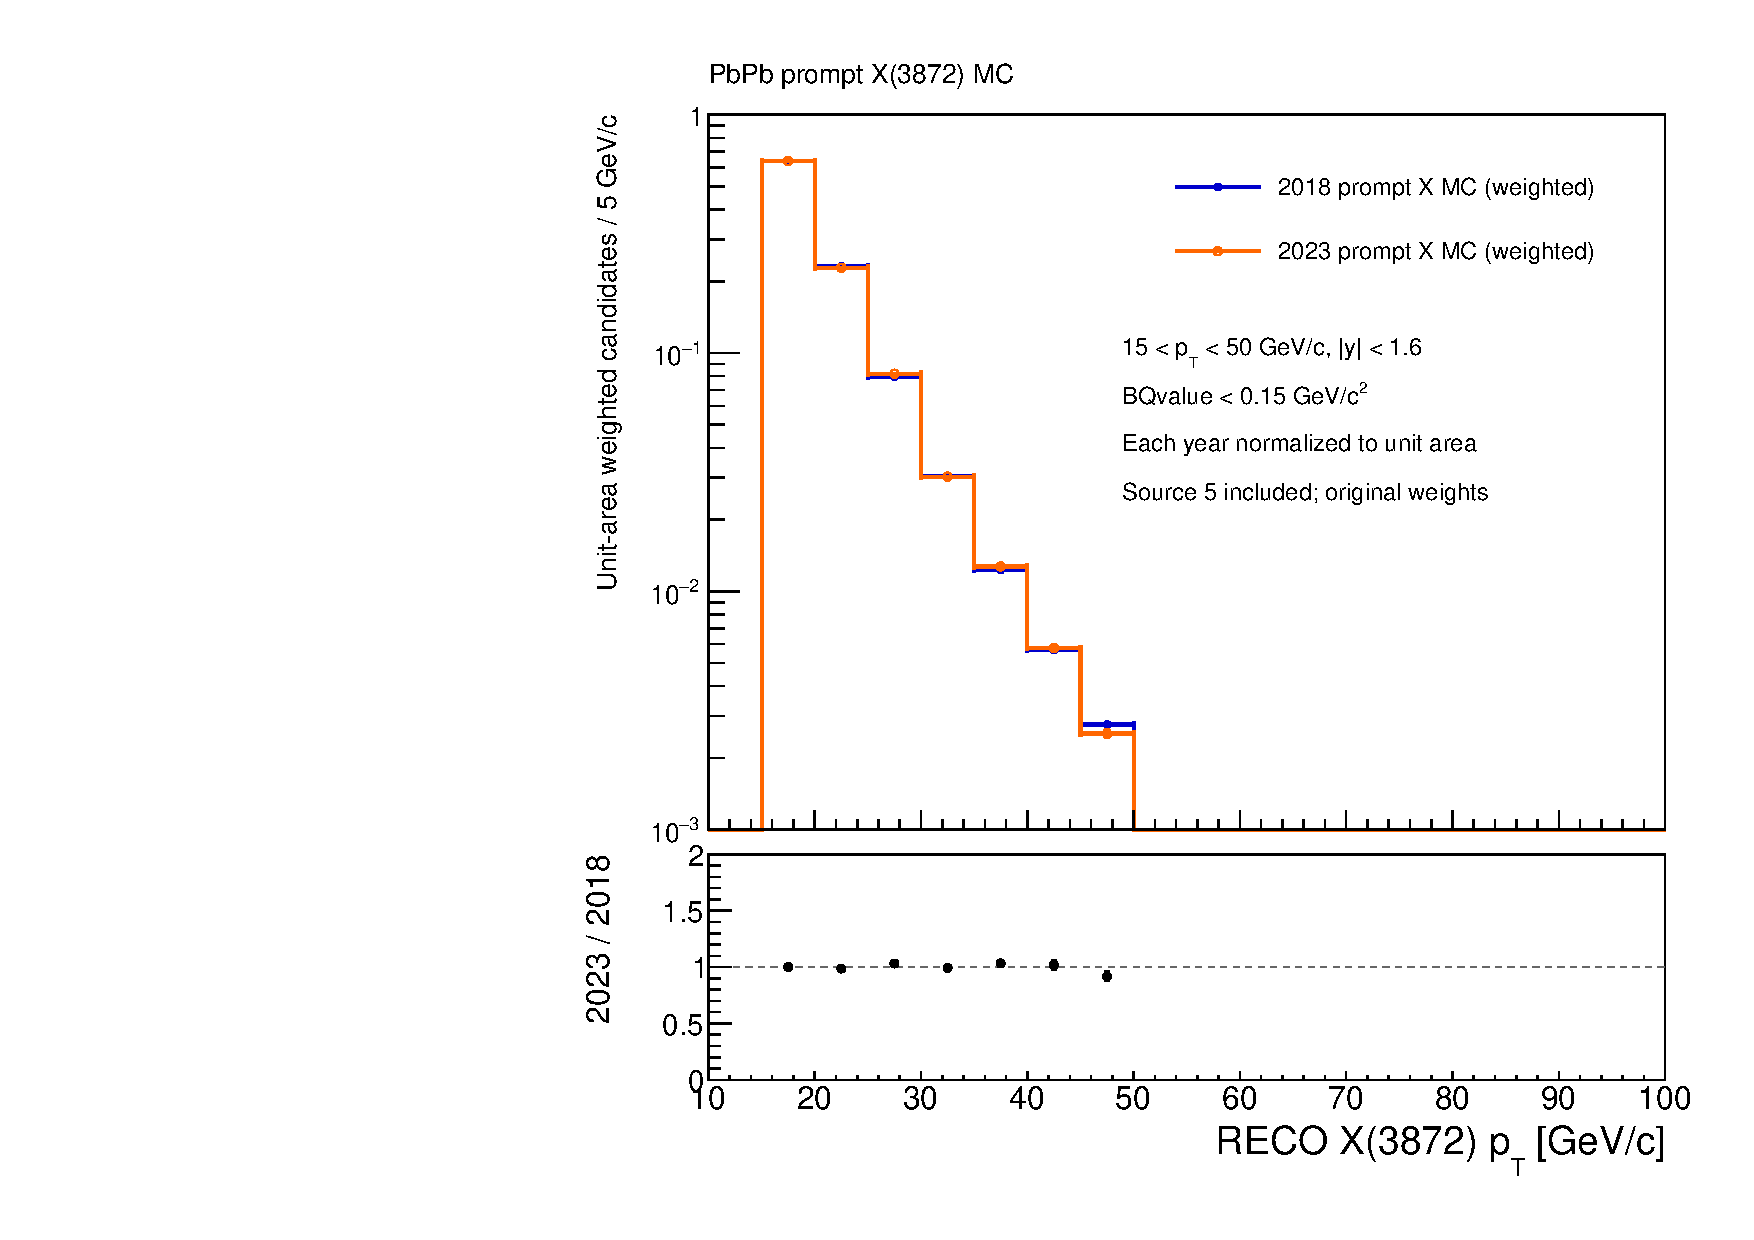
\includegraphics[width=\linewidth,height=0.75\textheight,keepaspectratio]{figures/20260930/fiducial_pt_pthat5_included.pdf}
\column{0.29\textwidth}\small
$15<\var{Bpt}<50$ GeV\par
$|\var{By}|<1.6$\par
$\var{BQvalue}<0.15$ GeV\par\medskip
\textbf{pthat 5 component included.}\par\medskip
Each year normalized to unit area after selection.\par\medskip
Although the pthat 5 component behaves differently in 2018 and 2023, the $p_T$ distributions after reweighting are very similar.
\end{columns}

\end{frame}



